\documentclass[11pt,a4paper]{article}

\usepackage{../../templates/style}

\begin{document}

\begin{problem}{Skyline}{standard input}{standard output}{1 second}{64 megabytes}

รัฐบาลวางแผนสร้างเมืองใหม่บนพื้นที่ราบที่มีระดับเสมอกัน โดยกำหนดให้อาคารที่จะสร้างแต่ละหลังมีรูปทรงเป็นสี่เหลี่ยมผืนผ้า หลังจากที่มีการสร้างอาคารแล้วเมื่อมองตัวเมืองจากระยะไกล จะเห็นเส้นขอบฟ้าตามแนวเส้นขอบของอาคาร และทุกครั้งที่มีการสร้างอาคารเพิ่มขึ้น เส้นขอบฟ้าของตัวเมืองจะเปลี่ยนแปลงไป

อาคารที่จะสร้างขึ้นแต่ละหลัง กำหนดด้วยจำนวนเต็มบวกสามจำนวนคือ $( L_i , H_i , R_i )$ เมื่อ $L_i$ และ $R_i$ เป็นตำแหน่งตามแกนนอนด้านซ้ายและขวาของอาคารลำดับที่ $i$ ตามลำดับ ส่วน $H_i$ เป็นความสูงของอาคารนั้น เช่น $(1, 11, 5)$ หมายถึง อาคารที่สร้างขึ้นโดยมีขอบด้านซ้ายอยู่ที่ตำแหน่งที่ $1$ ขอบด้านขวาอยู่ที่ตำแหน่งที่ $5$ ของแกนนอน และมีความสูงเป็น $11$ หน่วย เมื่อสร้างอาคารนี้เสร็จจะได้เส้นขอบฟ้าใหม่เป็น $(1, 11, 5, 0)$ นั่นคือ ที่ตำแหน่งที่ $1$ ขอบฟ้ายกขึ้นสูง $11$ หน่วยตามความสูงของอาคารไปจนถึงตำแหน่งที่ $5$ แล้วความสูงลดลงเป็น $0$

\begin{figure}[h]
\centering
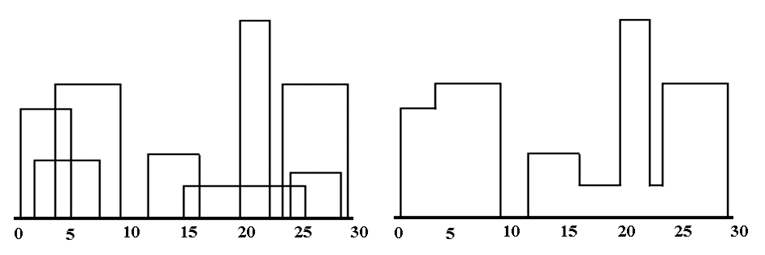
\includegraphics[width=0.8\textwidth]{../latex/img/1008/1008-1.png}
\caption{ตัวอย่างการสร้างอาคารที่เป็นไปได้ และเส้นขอบฟ้าที่สังเกตได้}
\end{figure}


แผนภาพด้านซ้ายมือแสดงตัวอย่างเมืองที่มีการสร้างอาคารแล้ว $8$ หลัง ซึ่งอาคารแต่ละหลังมีข้อมูลดังนี้ $(1, 11, 5), (2, 6, 7),$ $(12, 7, 16), (14, 3, 25), (19, 18, 22), (3, 13, 9), (23, 13, 29)$ และ $(24, 4, 28)$ ทำให้เกิดเส้นขอบฟ้าใหม่ตามแผนภาพด้านขวามือ ซึ่งแทนด้วยลำดับตัวเลขดังนี้ $(1, 11, 3, 13, 9,0, 12, 7,16, 3, 19,18, 22,3, 23,13, 29,0)$ 


\underline{\textbf{โจทย์}} จงเขียนโปรแกรมคำนวณหาเส้นขอบฟ้าจากข้อมูลของอาคารที่กำหนดให้ และแสดงผล

\InputFile

\textbf{บรรทัดแรก}  รับค่า $N$ แทนจำนวนอาคารที่ต้องการหาเส้นขอบฟ้า โดยที่ $1 \leq N \leq 2\,500$ 

\textbf{บรรทัดที่ 2 ถึง $N+1$}  บรรทัดที่ $i$ ให้รับค่า $L_i$ $H_i$ $R_i$ ระหว่างข้อมูลแต่ละตัวคั่นด้วยเว้นวรรค $1$ วรรค แทนตำแหน่งตามแกนนอนด้านซ้าย ความสูง และตำแหน่งตามแกนนอนด้านขวาของอาคารลำดับที่ $i$ ตามลำดับ โดยที่ $1 \leq L_i , H_i , R_i \leq 255$ 

\OutputFile

\textbf{มีบรรทัดเดียว} ให้แสดงข้อมูลเส้นขอบฟ้าที่เกิดจากข้อมูลของอาคาร โดยเส้นขอบฟ้ามีรูปแบบดังนี้: $v_1$ $v_2$ $v_3$ $…$ $v_{n-2}$ $v_{n-1}$ $v_n$ (แต่ละจำนวนให้คั่นด้วยเว้นวรรค $1$ วรรค) โดยเมื่อ $i$ เป็นจำนวนคี่ $v_i$ จะแทนตำแหน่งของเส้นขอบฟ้าตามแกนนอน และเมื่อ $i$ เป็นจำนวนคู่ $v_i$ แทนความสูงของเส้นขอบฟ้าที่ตำแหน่งนั้น (ด้วยเหตุนี้ $v_n$ จึงมีค่าเป็น $0$ เนื่องจากเส้นขอบฟ้าลดลงสู่ระดับพื้น)
\Examples

\begin{example}
\exmp{2
1  11  5
2  6  7}{1 11 5 6 7 0}%
\exmp{8
1  11  5
2  6  7
12  7  16
14  3  25
19  18  22
3  13  9
23  13  29
24  4  28}{1 11 3 13 9 0 12 7 16 3 19 18 22 3 23 13 29 0}%
\end{example}

\Source

การแข่งขันคอมพิวเตอร์โอลิมปิก สอวน. ครั้งที่ 2 มหาวิทยาลัยบูรพา

\end{problem}

\end{document}